\documentclass[referat]{SCWorks}

\usepackage{preamble}

\begin{document}

% Кафедра (в родительном падеже)
\chair{математической кибернетики и компьютерных наук}

% Тема работы
\title{Компьютерная графика}

% Курс
\course{1}

% Группа
\group{111}

% Специальность/направление код - наименование
\napravlenie{02.03.02 "--- Фундаментальная информатика и информационные технологии}

\studenttitle{студентов}

% Фамилия, имя, отчество в родительном падеже
\author{Алексеева Никиты Игоревича \\ Зинченко Елены Валентиновны \\ Неклюдовой Марины Сергеевны}

% Научный руководитель (для реферата преподаватель проверяющий работу)
\satitle{доцент, к.\,пед.\,н.} % должность, степень, звание
\saname{А.\,П.\,Грецова}

% Год выполнения отчета
\date{2025}

\maketitle

% Включение нумерации рисунков, формул и таблиц по разделам (по умолчанию -
% нумерация сквозная) (допускается оба вида нумерации)
\secNumbering

\tableofcontents

\intro

% текст

\section{Основы компьютерной графики}

\subsection{Введение в компьютерную графику}

% текст

\subsection{Типы компьютерной графики}

% текст

\subsection{Математические основы}

% текст

\subsection{Этапы рендеринга}

% текст

\section{Инструменты и библиотеки C++ для графики}

\subsection{Обзор популярных библиотек}

\textbf{Графические библиотеки} "--- это наборы заранее написанного кода, которые упрощают процесс отрисовки графики в приложениях. Они предоставляют набор функций для выполнения распространённых графических задач, что значительно сокращает объём шаблонного кода, который приходится писать разработчикам. Также они позволяют программистам сосредоточиться на разработке своих приложений, а не на низкоуровневых деталях рендеринга графики.

Существует множество разных графических библиотек, каждая из которых имеет свои плюсы и минусы, а также подходит для определённых задач. Поэтому для решения вашей задачи для начала нужно определиться с библиотекой, зная её преимущества и недостатки. Перечислим примеры таких библиотек для C++ и остановимся на некоторых из них, чтобы рассмотреть их подробнее \cite{graphics_libraries}:
\begin{itemize}
    \item SDL;
    \item SFML;
    \item OpenGL;
    \item Allegro;
    \item Juce;
    \item Qt и другие.
\end{itemize}

\textbf{SFML} (Simple and Fast Multimedia Library) "--- это одна из самых быстрых и простых библиотек C++ для реализации 2D"=графики, которая является мультимедийной и позволяет работать с системой, непосредственно с графикой, окнами, аудио и сетью, что помогает упростить разработку игр и мультимедийных приложений. Кроме того она является мультиплатформенной и может быть запущена на распространённых операционных системах: Windows, Linux, macOS, Android и iOS. SFML представленна и на других языках кроме C++: C, .NET, Java, Ruby, Python, Go и других, что позволяет расширить использование данной библиотеки в разных проектах. \cite{sfml_doc}

Стоит выделить главные преимущества SFML:
\begin{itemize}
    \item объектно-ориентированный дизайн, упрощающий использование и понимание;
    \item встроенная поддержка различных графических элементов, таких как фигуры, спрайты и текст;
    \item отлично подходит для начинающих и небольших и средних проектов.
\end{itemize}

\textbf{SDL} (Simple DirectMedia Layer) "--- это кроссплатформенная библиотека для разработки, предназначенная для низкоуровневого доступа к аудио, элементам ввода и графическому оборудованию. SDL поддерживается на всех доступных платформах (Windows, macOS, Linux, iOS и Android), а также возможно использование на разных языках: C\#, Python, Rust и другие. Используется библиотека для разработки игр, видеоплееров и других мультимедийных приложений. \cite{sdl_doc}

Некоторые возможности SDL:
\begin{itemize}
    \item аппаратно-ускоренный вывод 2D- и 3D-графики;
    \item простота интеграции с другими библиотеками, такими как OpenGL, \\ Direct3D или Vulkan;
    \item поддержка шейдеров, текстур и других средств работы с графикой. 
\end{itemize}

\textbf{OpenGL} (Open Graphics Library) "--- это библиотека, которая является одной из самых популярных графических \textbf{прикладных программных интерфейсов} (API – Application Programming Interface) для разработки приложений в области 2D"= и 3D"=графики. Она была разработана ещё в 1992 году на основе библиотеки IRIS GL и до 2017 года активно поддерживалась и развивалась до появления Vulkan API. Однако OpenGL всё ещё широко применяется в различных сферах. Стоит отметить, что библиотека сложнее SFML и SDL, но предлагает широкие возможности и гибкость для продвинутых графических приложений. \cite{opengl_doc}

Рассмотрим особеннсоти OpenGL.
\begin{itemize}
    \item \textit{Стабильность.} Дополнения и изменения реализуются таким образом, чтобы сохранить совместимость с разработанным ранее программным обеспечением.
    \item \textit{Мультиплатформенность} Приложения, использующие OpenGL, гарантируют одинаковый визуальный результат вне зависимости от типа используемой операционной системы и организации отображения информации. Кроме того, эти приложения могут выполняться как на персональных компьютерах, так и на рабочих станциях и суперкомпьютерах.
    \item \textit{Легкость применения.} Стандарт OpenGL имеет продуманную структуру и интуитивно понятный интерфейс, что позволяет с меньшими затратами создавать эффективные приложения, содержащие меньше строк кода, чем с использованием других графических библиотек.
\end{itemize}

\subsection{Настройка среды разработки}

% текст

\subsection{Практические примеры на SFML}

% Познакомимся с библиотекой SFML на простых практических примерах. Для этого нужно скачать бибилотеку на компьютер с официального сайта: \url{https://www.sfml-dev.org/download/}, затем понадобиться провести подключение всех компонентов библиотеки в рабочую область.

Рассмотрим простейшие функции, которые помогут написать первую тестовую программу (вывод простых фигур на экран). Для начала понадобится подключить заголовочный файл, позволяющий работать непосредственно с графикой:

\begin{lstlisting}[style=myStyle, numbers=none]
#include <SFML/Graphics.hpp>
\end{lstlisting}

После подключения появляется возможность использовать новые функции. В \texttt{main} инициализируем новое окно размером 800 на 600 пикселей следующим образом:

\begin{lstlisting}[style=myStyle, numbers=none]
sf::RenderWindow window(sf::VideoMode(800, 600), "Shapes");
\end{lstlisting}

Теперь определимся с формой, размером, цветом и позицией отображаемых фигур и инициализируем их, задав нужные параметры с помощью простых и интуитивно понятных методов:

\begin{lstlisting}[style=myStyle]
sf::CircleShape circle(50.f);
circle.setFillColor(sf::Color::Red);
circle.setPosition(100.f, 100.f);

sf::RectangleShape rect(sf::Vector2f(120.f, 60.f));
rect.setFillColor(sf::Color::Blue);
rect.setPosition(300.f, 200.f);
\end{lstlisting}

После инициализации всех необходимых элементов можно приступить к созданию \textbf{основного цикла}, который реализует всю логику программы и обеспечивает её работу. Он включает в себя такие этапы как: обработка событий, обновление логики, отрисовка. В нашей программе отсутствует логика, поэтому мы пропускаем второй этап:

\begin{lstlisting}[style=myStyle]
while (window.isOpen()) {
    sf::Event event;
    while (window.pollEvent(event)) {
        if (event.type == sf::Event::Closed)
            window.close();
    }

    window.clear(sf::Color::Black);
    window.draw(circle);
    window.draw(rect);
    window.display();
}
\end{lstlisting}

Обязательным элементом является наличие цикла, обрабатывающего события "--- \texttt{\color{blue}while} \texttt{window.pollEvent(event)}, если бы его не было, то программу было бы невозможно просто так закрыть. Полный код (\autoref{lst:shapes}) и результат программы (\autoref{fig:shapes}).
\begin{figure}[H]
    \centering
    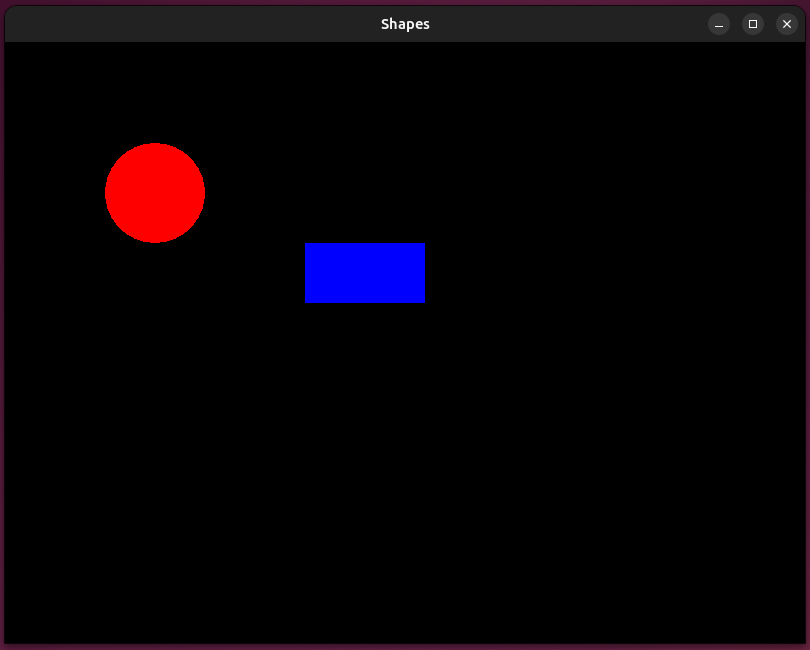
\includegraphics[width=0.8\textwidth]{src/img/sfml_shapes.png}
    \caption{Shapes}
    \label{fig:shapes}
\end{figure}

Рассмотрим обработку событий чуть подробнее. Пока запущено окно, оно постоянно проверяет было ли совершено какое-либо событие (нажатие клавиши, движение мыши и другие), если такое событие нашлось, то оно помещяется в очередь событий. Затем методом \texttt{pollEvent(event)} для окна мы вытаскиваем событие из очереди и присваиваем его переменной \texttt{event} класса \texttt{sf::Event}. После чего обрабатываем его и переходим к  следующему событию в случае, если очередь не пуста. Рассмотрим на примере движения мыши и нажатия клавиши \texttt{Escape}:

\begin{lstlisting}[style=myStyle]
if (event.type == sf::Event::KeyPressed) {
    if (event.key.code == sf::Keyboard::Escape)
        window.close();
}

if (event.type == sf::Event::MouseMoved) {
    std::cout << "Mouse position: " << event.mouseMove.x << ", " << event.mouseMove.y << std::endl;
}
\end{lstlisting}

Предварительно подключив заголовочный файл \texttt{iostream}, в результате получим, что при движении мыши в терминале будет обновляться её позиция, а по нажатию клавиши \texttt{Escape} программа завершится. Полный код (\autoref{lst:events}) и резульат (\autoref{fig:events}).
\begin{figure}[H]
    \centering
    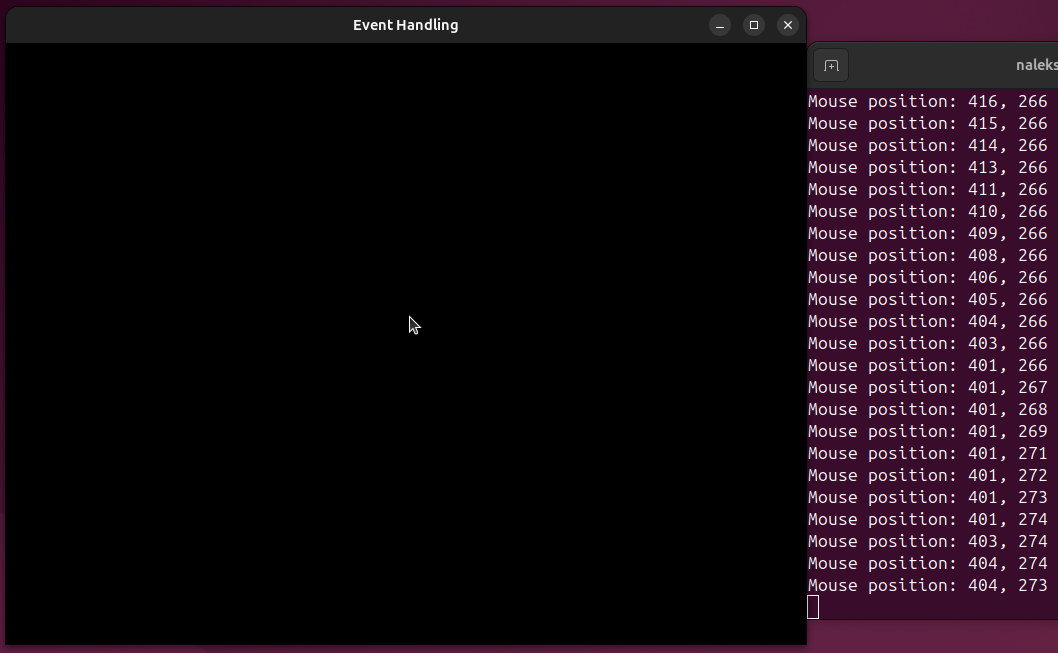
\includegraphics[width=0.8\textwidth]{src/img/sfml_events.png}
    \caption{Events}
    \label{fig:events}
\end{figure}

Последнее, что хотелось бы рассмотреть "--- это движение спрайта. В качестве последнего будет выступать круг, который мы уже умеем инициализировать и отображать. Реализуем самый простой способ движения "--- каждый кадр будем смещать спрайт на \texttt{X} и \texttt{Y} пикселей с помощью метода \texttt{move(X, Y)}. Для этого инициализируем нужные переменные и в основном цикле сдвинем спрайт:

\begin{lstlisting}[style=myStyle]
float speedX = 2.5f, speedY = 2.f;
ball.move(speedX, speedY);
\end{lstlisting}

Для того, чтобы постоянно в кадре наблюдать движение спрайта, пропишем простую логику. Пускай круг будет \flqq отскакивать\frqq\ от границ окна:

\begin{lstlisting}[style=myStyle]
if (ball.getPosition().x <= 0 || ball.getPosition().x >= 800 - 60) speedX = -speedX;
if (ball.getPosition().y <= 0 || ball.getPosition().y >= 600 - 60) speedY = -speedY;
\end{lstlisting}

Теперь мы можем постоянно наблюдать, как круг движется и \flqq ударяется\frqq\ о границы окна. На \autoref{fig:animation} светлым цветом показана текущая позиция круга, а на тёмных "--- позиции, которые он прошёл. В итоге движение получилось неидальным. Чтобы его улучшить (сделать более плавным) можно ограничить частоту кадров методом \texttt{setFramerateLimit()} для окна, а самый главный способ "--- преобразовать скорость из значения за кадр в значение, не зависящее от частоты кадров в секунду (\autoref{lst:animation}).
\begin{figure}[H]
    \centering
    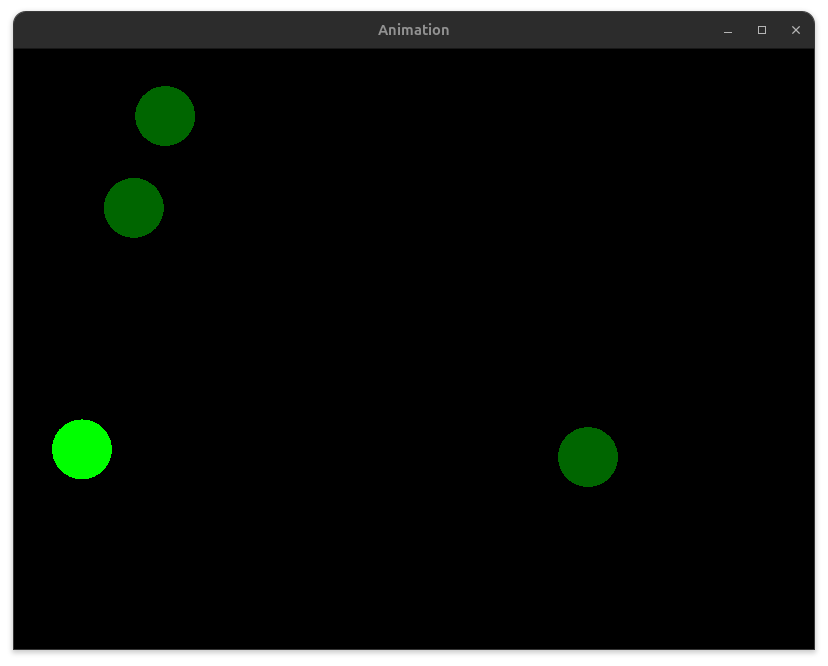
\includegraphics[width=0.8\textwidth]{src/img/sfml_animation.png}
    \caption{Animation}
    \label{fig:animation}
\end{figure}

\subsection{Переход к 3D: основы OpenGL}

% \input{src/section2/opengl.tex}

\section{Реализация графических алгоритмов}

\subsection{Алгоритмы растеризации}

% текст

\subsection{Заливка и работа с цветом}

% текст

\subsection{Оптимизация графики}

% текст

\conclusion

% текст

% Отобразить все источники. Даже те, на которые нет ссылок.
% \nocite{*}

\bibliographystyle{ugost2003}
\bibliography{thesis}

% Окончание основного документа и начало приложений Каждая последующая секция
% документа будет являться приложением
\appendix

\end{document}
